%
% JFFS3 design issues.
%
% Copyright (C), 2005, Artem B. Bityutskiy, <dedekind@infradead.org>
%
% $Id: intro.tex,v 1.5 2005/11/27 14:37:50 dedekind Exp $
%

The main idea how to fix in JFFS2 to make it scalable is \emph{to move the
index from RAM to flash}. Unfortunately, this requires complete JFFS2 redesign
and \mbox{re-implementation} and the design of JFFS3 is largely different to
the design of JFFS2. This section discusses the base JFFS3 design ideas without
any detailed description.

%
% INDEXING PROBLEM
%
\subsection{Indexing problem}

There is a large difference between block devices and flash devices in how they
allow to update the contents of a sector. Block devices admit of
\mbox{so-called} "\emph{\mbox{in-place} updates}", i.e. the update may be
written straight to the sector. Flash devices do not allow this unless the
whole eraseblock has been erased before.

Obviously, it is unacceptable to erase the whole eraseblock each time a sector
is updated. Instead, \mbox{so-called} "\emph{\mbox{out-of-place} updates}"
technique is usually used. This simply means that no attempts to update
sectors \mbox{in-place} are made but instead, updates are written to some
other sector and the contents of the previous sector is afterwords regarded as
garbage.

This "\mbox{out-of-place} writes" property of flash devices assumes that JFFS3
also has \mbox{log-structured} design as in JFFS3 any update is written
\mbox{out-of-place}. And it seems that this is natural for any flash file
system to have log-structured design.

It is interesting to notice that in \mbox{log-structured} file systems for
block devices (like the one described in~[\ref{ref_LFS}]) not any update is
"\mbox{out-of-place}". There are always some \mbox{fixed-position} sectors
present. These sectors usually refer the file system index, admit of quick
file system mount and they are updated \mbox{in-place}.

But flash devices have limited number of erase cycles for each eraseblock and
it is impossible to guaranty good \mbox{wear-levelling} if some eraseblocks are
reserved for similar purposes. So, it is important that \emph{in JFFS3 there
are no \mbox{in-place} updates} as good \mbox{wear-levelling} is one of the
main requirements to JFFS3 (see section~\ref{ref_SectionJFFS3Req}).

The "\mbox{out-of-place} updates" property makes it difficult to maintain the
index on the flash media. Figure~\ref{ref_FigureIndexProblem} demonstrates why.

%
% Figure with index problem example
%
\begin{figure}[h]
\begin{center}
\begin{htmlonly}
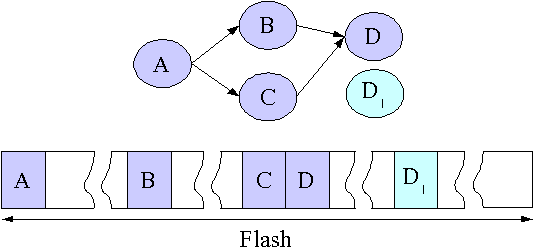
\includegraphics{pics/idxprobl.png}
\end{htmlonly}
%begin{latexonly}
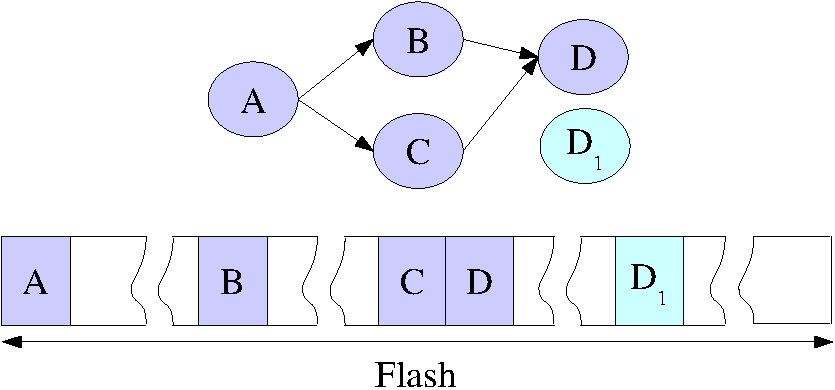
\includegraphics[width=90mm,height=45mm]{pics/idxprobl.pdf}
%end{latexonly}
\end{center}
\caption{JFFS3 indexing problem example.}
\label{ref_FigureIndexProblem}
\end{figure}

Suppose the index is kept and maintained on flash and it consists of 4
parts $A$, $B$, $C$, and $D$ which refer each other: $A$ refers $B$ and $C$,
$B$ refers $D$, and $C$ refers $D$. This means, that $A$ contains the physical
flash address of $B$ and $C$ and so on.

Suppose $D$ should be updated. Since it is updated \mbox{out-of-place}, the
newer version $D_1$ is written to some other place. But there are $B$ and $C$
which still refer $D$, not $D_1$, and they ought to be updated as well. And
when they are updated \mbox{out-of-place}, $A$ will still refer the old $B$ and
$C$, and so on. Thus, it is not that trivial to store and maintain indexing
information on the flash media.

%
% WANDERING TREES
%
\subsection{Wandering trees} \label{ref_SectionWandTrees}

To address the above problem it is possible to use \emph{wandering trees}.
Figure~\ref{ref_FigureWandtree} demonstrates how do wandering trees work.

%
% Figure with the wandering tree example
%
\begin{figure}[h]
\begin{center}
\begin{htmlonly}
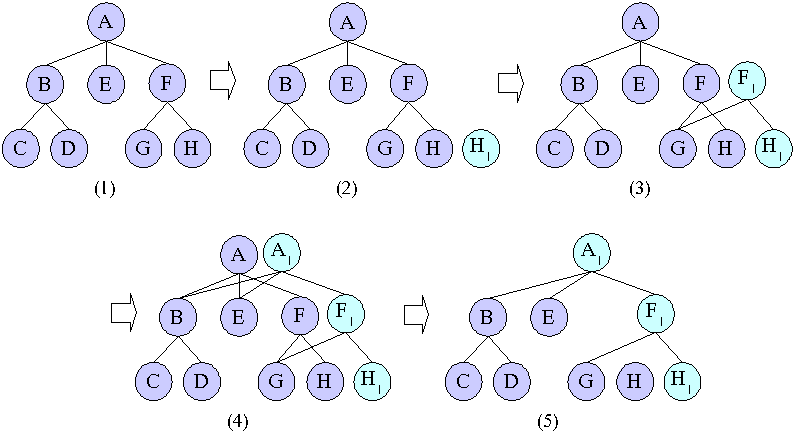
\includegraphics{pics/wandtree.png}
\end{htmlonly}
%begin{latexonly}
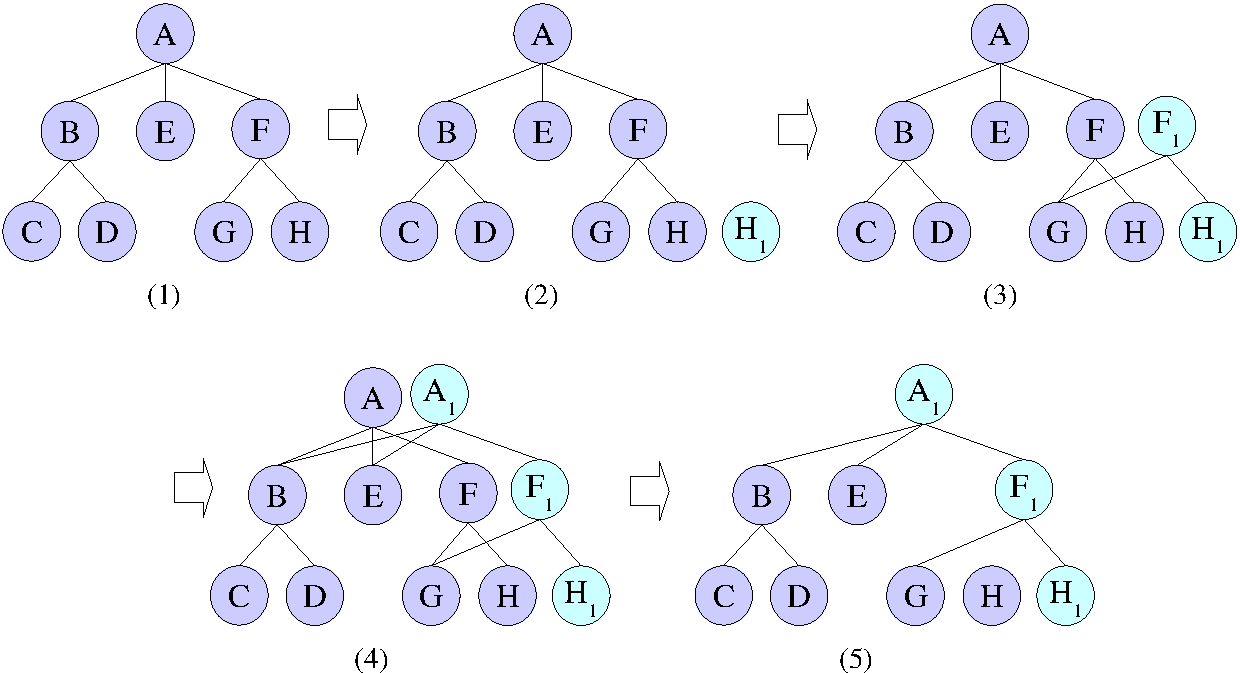
\includegraphics[width=159mm,height=80mm]{pics/wandtree.pdf}
%end{latexonly}
\end{center}
\caption{Wandering tree example.}
\label{ref_FigureWandtree}
\end{figure}

\begin{enumerate}

\item Suppose that the index is a tree and it is stored and maintained
on the flash media. The tree consists of nodes
$A$, $B$, $C$, $D$, $E$, $F$, $G$, and $H$.
Suppose node $H$ should be updated.

\item At first, the updated version $H_1$ is written. Obviously, $F$ still
refers $H$.

\item Now the corresponding link in node $F$ is changed and node $F_1$ is
written to flash. $F_1$ refers $H_1$. But as $F_1$ is also written
\mbox{out-of-place}, $A$ still refers the old node $F$.

\item Finally, the new root node $A_1$ is written ant it refers $F_1$.

\item Nodes $A$, $F$, $H$ are now treated as garbage and the updated tree is
composed by nodes $A_1$, $B$, $C$, $D$, $E$, $F_1$, $G$, and $H_1$.

\end{enumerate}

So, wandering trees is the base idea of how the indexing information is going
to be maintained on the flash media in JFFS3. And it stands to reason that any
tree may be called "wandering tree" if any update in the tree requires updating
parent nodes up to the root. For example, it makes sense to talk about
wandering \mbox{Red-Black} trees or wandering \mbox{$B^+$-trees} and so forth.

%
% B+ TREES
%
\subsection{B-trees} \label{ref_SectionBTrees}

JFFS3 uses \mbox{$B^+$-trees} and this subsection makes a short introduction to
\mbox{$B^+$-trees}. There is a plenty of books where one may find more
information. There are also many \mbox{on-line} resources available, e.g.
[\ref{ref_BTrees}].

The inexact definition of \mbox{$B$-tree} may be formulated as a balanced
search tree where each node may have many children. The \emph{branching factor}
or the \emph{fanout} defines the maximal number of node's children. While
\mbox{$B$-trees} may contain both useful data and \emph{keys} and \emph{links}
in \mbox{non-leaf} nodes, \mbox{$B^+$-trees} are \mbox{$B$-trees} which store
data only in leaf nodes, while \mbox{non-leaf} nodes contain only keys and
links.

%
% The figure with B+-tree example
%
\begin{figure}[h]
\begin{center}
\begin{htmlonly}
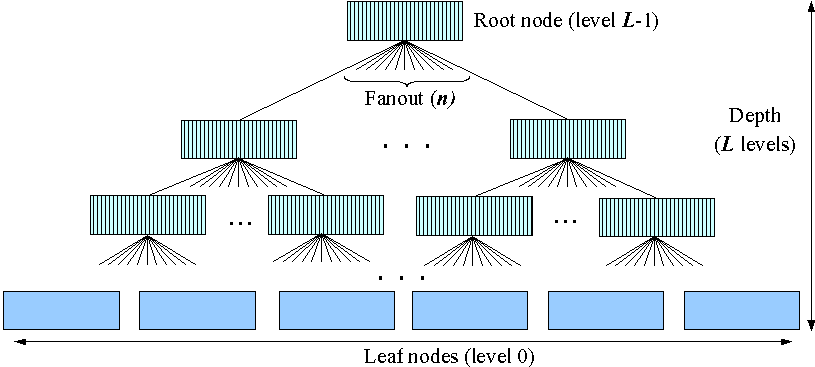
\includegraphics{pics/btree-01.png}
\end{htmlonly}
%begin{latexonly}
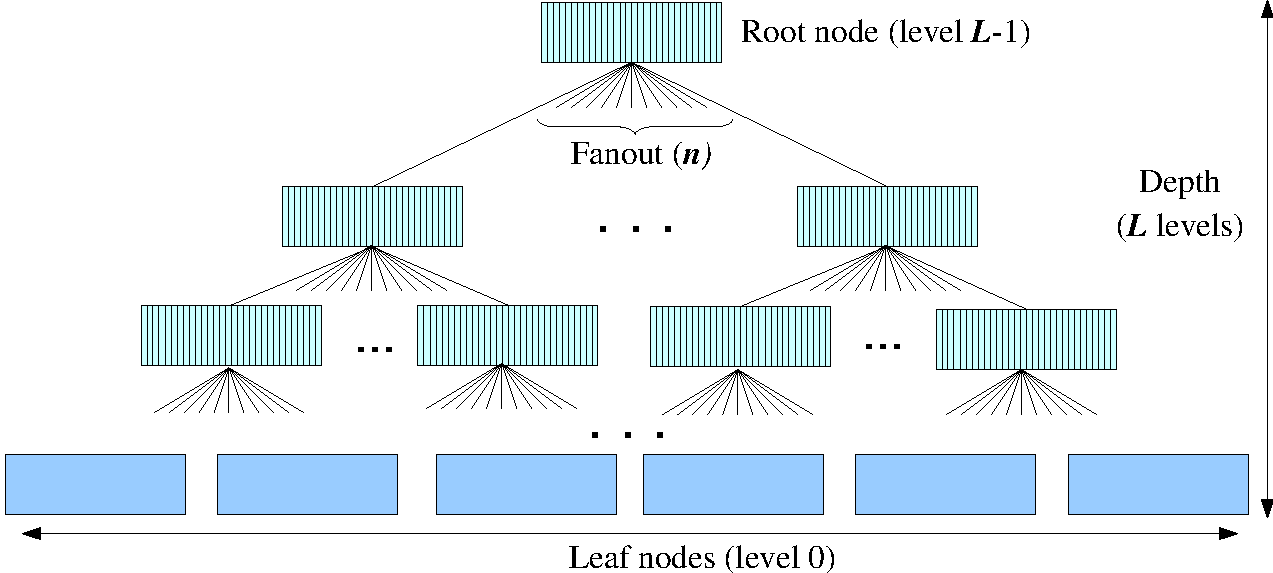
\includegraphics[width=159mm,height=65mm]{pics/btree-01.pdf}
%end{latexonly}
\end{center}
\caption{$B^+$-tree example.}
\label{ref_FigureBTree_01}
\end{figure}

Figure~\ref{ref_FigureBTree_01} demonstrates a \mbox{$B^+$-tree} with branching
factor $n$ and the number of level $L$. Note, that in JFFS3 levels are numbered
starting from \emph{leaf} nodes (level 0) and ending at the \emph{root} node
(level $L-1$).

Leaf nodes in the \mbox{$B^+$-tree} contain data which are indexed by
keys. \mbox{Non-leaf} nodes do not contain data, but contain only the indexing
information, namely, \emph{keys} and \emph{links}.

%
% Figure with B+-tree non-leaf node
%
\begin{figure}[h]
\begin{center}
\begin{htmlonly}
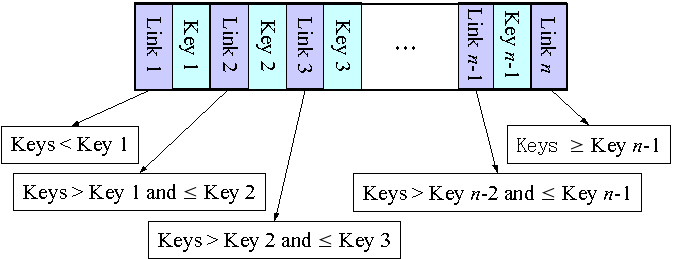
\includegraphics{pics/node-01.png}
\end{htmlonly}
%begin{latexonly}
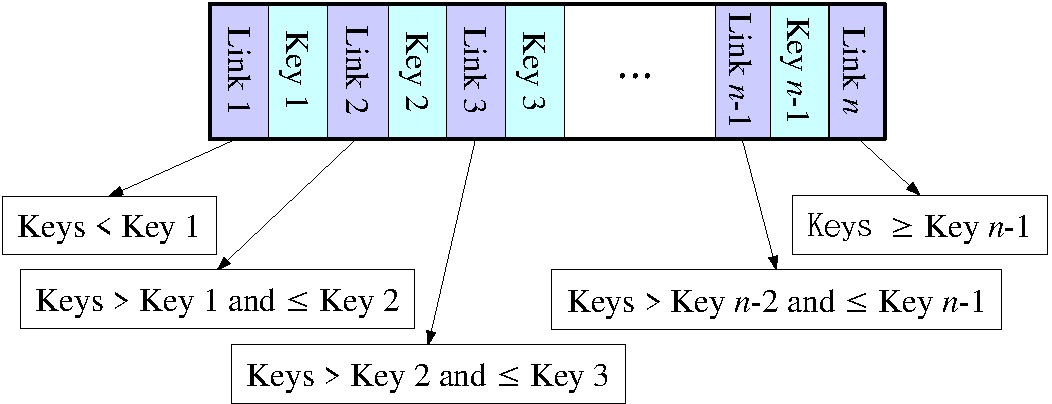
\includegraphics[width=160mm,height=60mm]{pics/node-01.pdf}
%end{latexonly}
\end{center}
\caption{The structure of a non-leaf node in $B^+$-tree.}
\label{ref_FigureNode_01}
\end{figure}

Figure~\ref{ref_FigureNode_01} depicts the structure of a \mbox{non-leaf}
node. There are $n$ links and $n-1$ keys in the node. Links may point to either
leaf nodes or other \mbox{non-leaf} nodes. In the former case, the leaf node
will contain data which corresponds to the key which follows the link. In the
latter case, the pointed \mbox{non-leaf} node (and the whole subtree with the
root in this \mbox{non-leaf} node) will contain more keys in range
$(Key~1, Key~2]$.

Keys are sorted in the ascending order in \mbox{non-leaf} nodes, so it is not
that difficult to lookup data corresponding to any key. Furthermore, the tree
is balanced, so the the number of lookup steps does not depend on the key.

When objects are inserted or removed from the tree, \mbox{re-balancing} may be
needed. The tree is \mbox{re-balanced} by means of splitting nodes or merging
them and there is a simple enough algorithm exists. Please, refer to Donald
Knuth's books for more information about \mbox{re-balancing}
\mbox{$B^+$-trees}.

\mbox{$B^+$-trees} are widely used when working with block devices (e.g., hard
drives). Indeed, these devices have a fixed input/output unit size (usually
referred to as a \emph{sector}) and it is natural to use \mbox{$B^+$-trees}
with node size multiple to the size of the sector in order to store information
on such devices.

%
% INDEXING IN JFFS3
%
\subsection{Indexing in JFFS3} \label{ref_SectionIndexing}

The way how JFFS3 stores and indexes the file system is similar to the approach
used by the \emph{Reiser4} file system (see~[\ref{ref_Reiser4}]). All the file
system objects (inodes, files, directory entries, extended attributes, etc) are
kept in one large \mbox{$B^+$-tree}. Effectively, the whole JFFS3 file system
may be regarded as one large \mbox{$B^+$-tree}. This tree is further referred
to just as "\emph{the tree}".

Every object which is stored in the tree has a \emph{key}, and objects are
found in the tree by their keys. To make it clearer what are object keys, the
following is an example of how they may look like:

\begin{itemize}

\item file data key: \{\texttt{inode number}, \texttt{offset}\};

\item directory entry key: \{\texttt{parent directory inode number},
\texttt{direntry name hash}\} and the like.

\end{itemize}

The following are terms which are used in JFFS3 to refer nodes of different
levels in the tree:

\begin{itemize}

\item nodes of level 0 are \emph{leaf nodes};

\item nodes of level 1 are \emph{twig nodes};

\item nodes which are not the root, not leaf, and not twig are \emph{branch
nodes};

\item \mbox{no-leaf} nodes (i.e., the root, branch and twig) are
\emph{indexing nodes}.

\end{itemize}

Note, the same terminology (except indexing nodes) is used in the Reiser4 file
system~[\ref{ref_Reiser4}].

\mbox{Non-leaf} nodes are called "indexing nodes" because they contain only
indexing information, nothing else. No file system data is kept in the indexing
nodes. Indexing nodes have fixed size which is equivalent to the flash
\emph{sector} size.

It is important to note that somewhat unusual terminology is used in this
document. The smallest input/output unit of the flash chip is called a
\emph{sector}. Since JFFS3 mainly orients to NAND flashes, the sector is mostly
the NAND page and is either 512 bytes or 2 Kilobytes. For other flash types the
sector may be different. If flash's minimal input/output unit is very small
(say, one bit as in case of NOR flash), there should be a layer which emulates
larger sectors (say, 512 bytes).

In opposite to indexing nodes, leaf nodes have flexible size, just like nodes
in JFFS2. So, roughly speaking, JFFS3 file system may be considered as JFFS2
file system (leaf nodes) plus indexing information (indexing nodes) (see
figure~\ref{ref_FigureBTree_02}). 

%
% Figure the JFFS3 tree example
%
\begin{figure}[h]
\begin{center}
\begin{htmlonly}
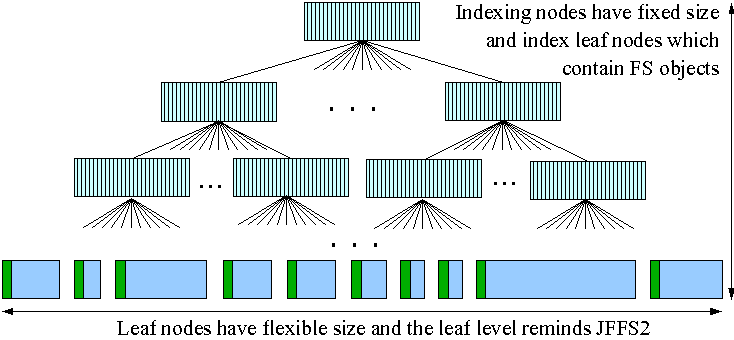
\includegraphics{pics/btree-02.png}
\end{htmlonly}
%begin{latexonly}
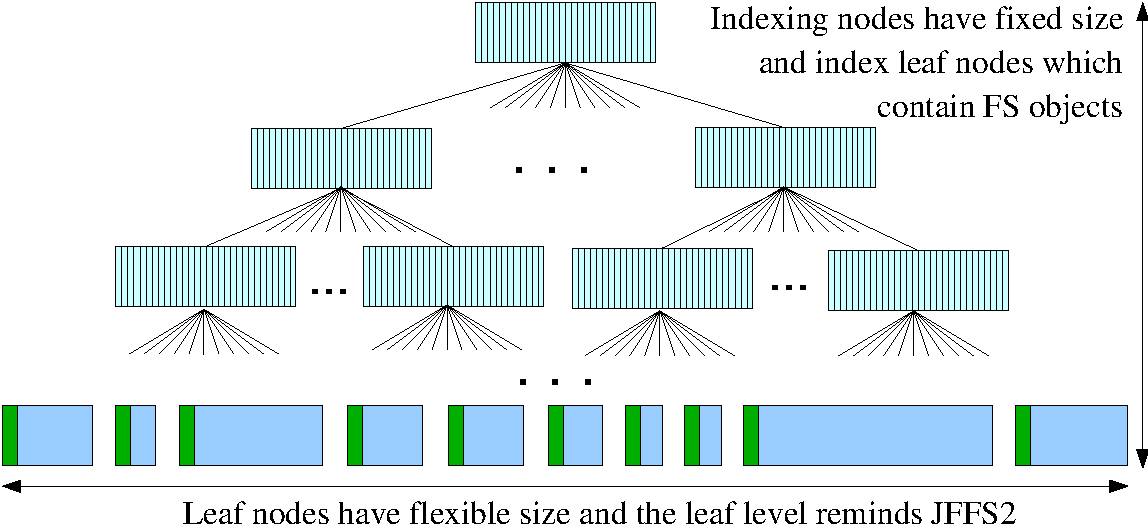
\includegraphics[width=159mm,height=65mm]{pics/btree-02.pdf}
%end{latexonly}
\end{center}
\caption{The JFFS3 tree.}
\label{ref_FigureBTree_02}
\end{figure}

Similarly to JFFS2, leaf nodes consist of \emph{header} and \emph{data}. The
header describes the node data and contains information like the key of the
node, the length, and the like. Node data contains some file system data, for
example a directory entry, file's contents, etc. 

Leaf and indexing nodes are physically separated, which means that there are
eraseblocks with only indexing nodes and with only leaf nodes. But of course,
this does not mean that the whole flash partition is divided on two parts, this
only means that the indexing and leaf nodes are not in one eraseblock.
Figure~\ref{ref_FigureFlash_01} illustrates this.

%
% Figure with demonstration leaf and indexing nodes separation.
%
\begin{figure}[h]
\begin{center}
\begin{htmlonly}
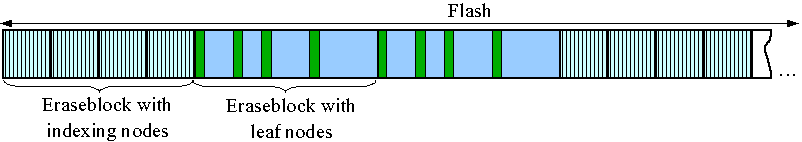
\includegraphics{pics/flash-01.png}
\end{htmlonly}
%begin{latexonly}
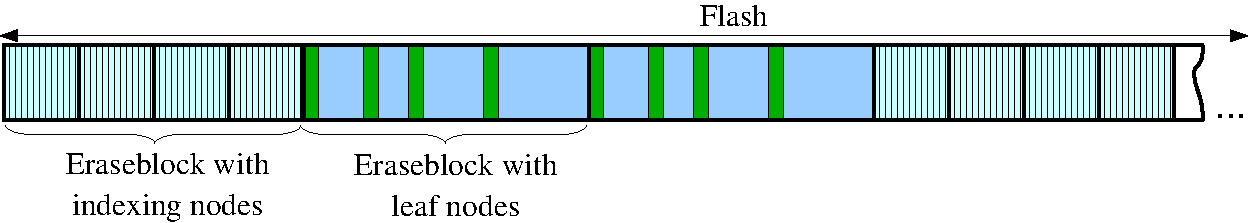
\includegraphics[width=159mm,height=25mm]{pics/flash-01.pdf}
%end{latexonly}
\end{center}
\caption{An illustration of leaf and indexing nodes separation.}
\label{ref_FigureFlash_01}
\end{figure}

Eraseblocks which contain only indexing nodes are called \emph{indexing
eraseblocks} and those with leaf nodes are called \emph{leaf eraseblocks}.

The depth of the tree depends on how many objects are kept in the file system.
The more files, directories, etc are present in the file system, the deeper is
the tree. Fortunately, the number of tree levels grows very slowly with the
growing number of file system objects and the tree lookup scales as
$O(log_n{S})$ (logarithmically).

The following are advantages of the JFFS3 indexing approach.

\begin{itemize}

\item Many different key assignment schemes may be used and this gives a
flexibility in how objects are sorted in the tree. Thus, one may optimize JFFS3
for specific workloads by means of changing the format of the keys.

\item Leaf nodes may be compressed, so JFFS3 admits of the \mbox{on-flight}
compression.

\item In case of corruptions of the indexing information it is possible to
\mbox{re-create} it by means of scanning leaf nodes' headers.

\item There is a clear separation between data and indexing information. This
implies that the indexing information and data may be cached separately,
without overlapping in the same cache lines. This leads to better cache usage
as described in the Reiser4 paper~[\ref{ref_Reiser4}].

\end{itemize}

%
% INDEXING EXAMPLE
%
\subsection{Indexing example}

This section illustrates how does JFFS3 indexing work by means of a simple
example. The example is very rough but it shows JFFS3 indexing in action. It is
assumed that keys of direntries and data objects have the same layout that
is mentioned in section~\ref{ref_SectionIndexing}.

Suppose that user does the following:

\begin{enumerate}

\item mounts JFFS3 file system to "\texttt{/mnt/jffs3}" directory;

\item issues "\texttt{ls /mnt/jffs3}" command;

\item reads the contents of "\texttt{/mnt/jffs3/my\_file}" file.

\end{enumerate}

The following are comments about what is going on in JFFS3 during the above
steps.

\begin{enumerate}

\item During mount JFFS3 locates the position of the root node. This is done
with help of the JFFS3 \emph{superblock} which will be described later
(see section~\ref{ref_SectionSB}).

\item To get the list of directory entries in the root directory, JFFS3
looks~up all objects matching the \{\texttt{2},~$*$\} key pattern. Indeed,
direntry keys have \{\texttt{parent~inode~\#},~\texttt{name~hash}\} format, the
root directory inode number is 2 (or another predefined constant).  $*$" means
wildcard. Thus, JFFS3, \{\texttt{2},~$*$\} will match to any direntry in the
root directory.

\item To read the "\texttt{my\_file}" file, JFFS3 first needs to find out its
inode number. The inode number is stored in the directory entry object. Hence,
JFFS3 reads \texttt{my\_file}'s direntry using
\{\texttt{1},~$H($\texttt{"my\_file"$)$}\} key ($H()$ is the hash function).

Then JFFS3 searches for \texttt{my\_file}'s data objects using
\{$I$,~\texttt{offset}\} keys. Depending on which part of file should be read,
\texttt{offset} may take different values.

\end{enumerate}

The above description is somewhat simplified e.g., JFFS3 also needs to read
\texttt{my\_file}'s attr-data object to fetch the inode length from there (see
section \ref{ref_SectionObjects}), etc. But the aim of the section is just to
provide an idea of how JFFS3 indexing works.

%
% THE JOURNAL
%
\subsection{The Journal} \label{ref_SectionJournalIntro}

The JFFS3 tree is both \mbox{$B^+$-tree} and wandering tree. Any file system
change implies that a new node is written to the flash media, which in turn,
assumes that a number of indexing nodes must be updated. Namely, the whole path
of indexing nodes up to the root node should be updated (see
section~\ref{ref_SectionWandTrees}).

Evidently, it is very expensive to update several indexing nodes on each file
system change and \emph{the journal} provides a mechanism to avoid this.

The journal consists of a set of eraseblocks (the \emph{journal eraseblocks})
which do not have a fixed location on flash and are not contiguous on flash.
Any flash eraseblock may be used as an journal eraseblock.

%
% Figure with journal illustration
%
\begin{figure}[h]
\begin{center}
\begin{htmlonly}
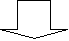
\includegraphics{pics/journal-01.png}
\end{htmlonly}
%begin{latexonly}
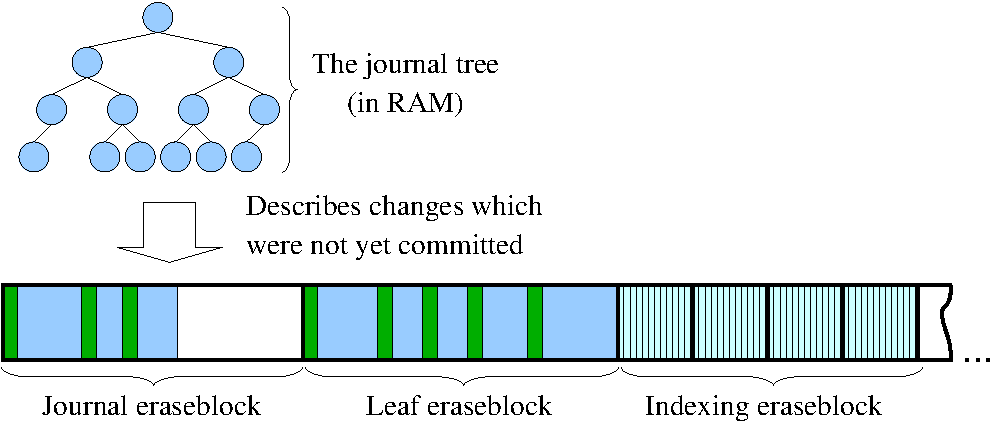
\includegraphics[width=159mm,height=60mm]{pics/journal-01.pdf}
%end{latexonly}
\end{center}
\caption{The JFFS3 journal.}
\label{ref_FigureJournal_01}
\end{figure}

When something is changed in the JFFS3 file system, the corresponding leaf node
is written to the journal, but the corresponding indexing nodes are not
updated. Instead, JFFS3 keeps track of file system changes in RAM in a data
structure called \emph{the journal tree} (see
figure~\ref{ref_FigureJournal_01}).

When something is read from the file system, JFFS3 first glimpses at the
\mbox{in-RAM} journal tree to figure out if the needed data is in the journal.
If the data are there, the journal is read, otherwise JFFS3 performs the usual
tree lookup (see figure~\ref{ref_FigureJournal_02}).

%
% Figure with write request
%
\begin{figure}[h]
\begin{center}
\begin{htmlonly}
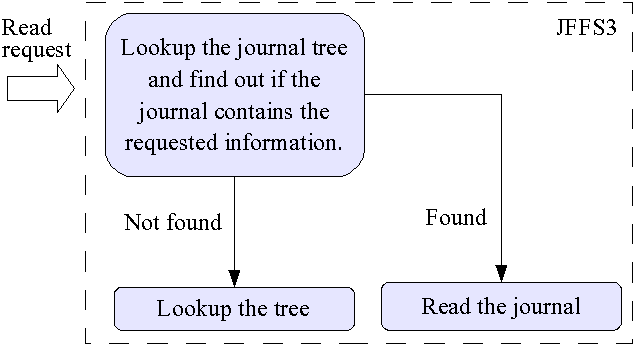
\includegraphics{pics/journal-02.png}
\end{htmlonly}
%begin{latexonly}
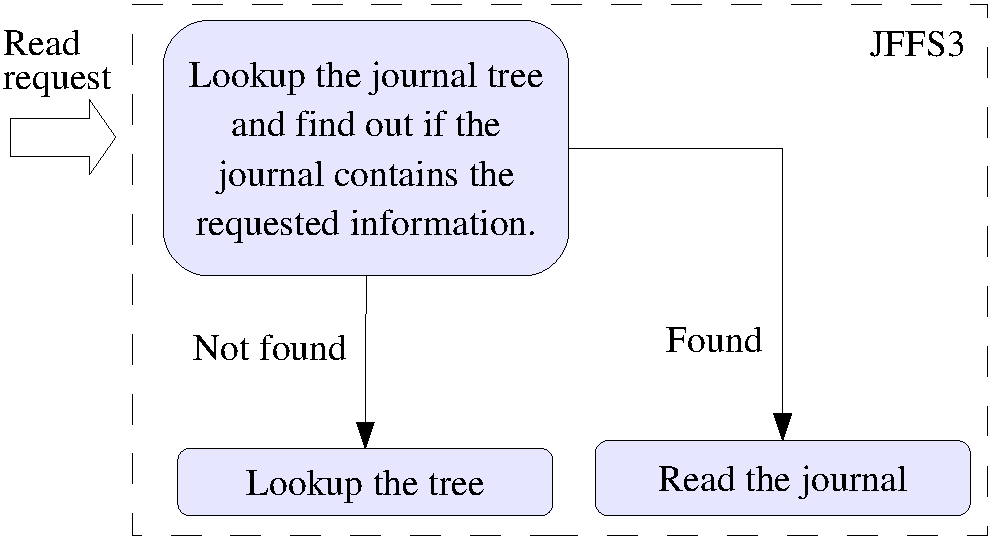
\includegraphics[width=120mm,height=55mm]{pics/journal-02.pdf}
%end{latexonly}
\end{center}
\caption{Read request processing in JFFS3.}
\label{ref_FigureJournal_02}
\end{figure}

The journal is \emph{committed} when it is full or in some other appropriate
for JFFS3 time. This means, that the indexing nodes corresponding to the
journal changes are updated and written to the flash. The committed
journal eraseblocks are then treated as leaf eraseblocks and new journal
eraseblocks are picked by JFFS3 using the common JFFS3
\mbox{wear-levelling} algorithm.

The journal makes it possible to postpone indexing information updates to later
and potentially more appropriate time. It also allows to merge many indexing
node updates and lessen the amount of flash write operations.

When JFFS3 file system is being mounted, the journal should be read, "replayed"
and the journal tree should be built. So, the larger is the journal, the longer
it may take to mount JFFS3. From the other hand, the larger is the journal, the
more writes may be deferred and the better performance may be achieved. By the
other words, there is a \mbox{trade-off} between the mount time and the
performance and one may vary these characteristics by means of changing the
size of the journal.

%
% GARBAGE COLLECTION
%
\subsection{Garbage collection}

Garbage collection is a vital part of any \mbox{log-structured} file system.
Over time, JFFS3 uses up all the flash free space and it needs to reclaim flash
space occupied by garbage. And the goal of Garbage Collector is to recycle
garbage and reclame flash space which it occupies. Since the only way to
reclaim it is to erase the whole eraseblock, Garbage Collector works in terms
of eraseblocks.

JFFS2 Garbage Collector is quite simple and works in several steps.

\begin{enumerate}

\item To reclaim dirt from an eraseblock, JFFS2 moves all valid nodes from this
eraseblock to another eraseblock.

\item As nodes have changed their positions, the JFFS2 \mbox{in-RAM} index is
adjusted.

\item The first eraseblock may be erased and \mbox{re-used}.

\end{enumerate}

Note, JFFS2 (and JFFS3) aways reserves several eraseblocks in order to
guarantee that there are always some free eraseblocks available to perform
garbage collection.

JFFS3 Garbage Collector is more complex. When valid data has been moved from an
eraseblock, the corresponding indexing nodes must be updated as well. Depending
on how many space Garbage Collector has reclaimed and how many space it has
spent to update indexing nodes, it might be that Garbage Collector produces
more garbage that it reclaims. This problem is demostrated in figure
\ref{ref_FigureGCProbl_01}.

%
% Figure wit hthe garbage collection problem
%
\begin{figure}[h]
\begin{center}
\begin{htmlonly}

\includegraphics{pics/gcprobl-01.png}
\end{htmlonly}
%begin{latexonly}
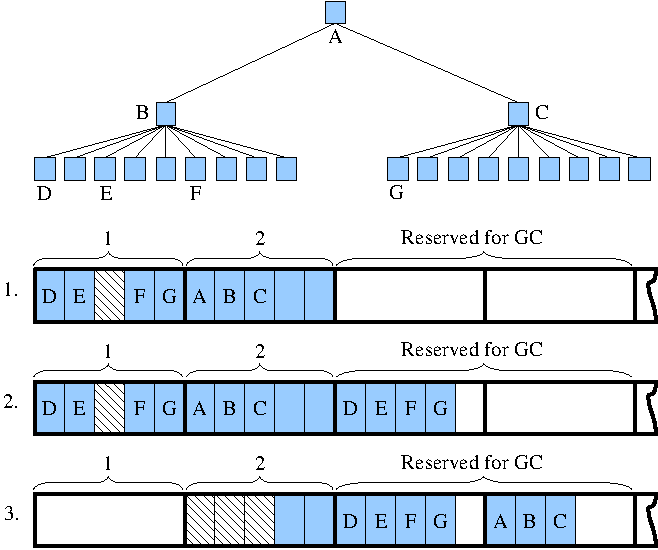
\includegraphics[width=120mm,height=96mm]{pics/gcprobl-01.pdf}
%end{latexonly}
\end{center}
\caption{JFFS3 garbage collection problem illustration.}
\label{ref_FigureGCProbl_01}
\end{figure}

There is a subtree with root in node $A$ depicted in the figure. At the
beginning (snapshot~1), leaf nodes $D$, $E$, $F$, and $G$ are situated in the
eraseblock number~1. Indexing nodes $A$, $B$, and $C$ are situated in the
eraseblock number~2. There are also two reserved eraseblocks. Suppose all nodes
have the same size equivlent to the size of sector which is 512 bytes in
this example.

At snapshot~2 JFFS3 has decided to reclaim 512 bytes of dirty space form
the eraseblock number~1. Garbage Collector moves all the valid nodes from the
eraseblock number~1 to one of the reserved eraseblocks. But as indexing nodes
$B$ and $C$ still refer old copies of the moved nodes in the eraseblock
number~1, this eraseblock cannot be erased so far. Indexing nodes $A$, $B$, and
$C$ have to be updated first.

At snapshot~3 Garbage Collector has updated indexing nodes $A$, $B$ and $C$,
putting them to one of the reserved eraseblocks. From now on, old copies of
nodes $A$, $B$, $C$, $D$, $E$, $F$, and $G$ at eraseblocks~1 and~2 comprise
garbage. The eraseblock number~1 was erased and is now free.

But unfortunatelly, the result is that Garbage Collector made more dirt that it
reclaimed space. Indeed, GC reclaimed 512 bytes while produced three times
greater amount of garbage (see the first three sectors at eraseblock~2,
snapshot~3). Compare snapshots~1 and~2.

Hence, it is obvious that garbage collection in JFFS3 is must be more complex
that in JFFS2. Chapter \ref{ref_SectionGC} discusses JFFS3 Garbage Collector in
details.

%
% THE SUPERBLOCK
%
\subsection{The superblock}

The JFFS3 \emph{superblock} is a data structure that describes the file system
as a whole and contains important information like the offset of the root node,
the journal eraseblocks, etc. When the file system is being mounted, it first
finds and reads the JFFS3 superblock.

In case of traditional file systems the superblock usually resides at a fixed
position on the disk and may be found very quickly. Conversely, due to the
"\mbox{out-of-place} write" flash property it is impossible to assign a fixed
position for the JFFS3 superblock. Things are getting even more complex because
of the need to provide good \mbox{wear-levelling}~-- it is incorrect to just
reserve several erasable blocks for the superblock unless it is guaranteed that
these eraseblocks will not be worn out earlier then the other eraseblocks.

We have the following two requirements that ought to be met in JFFS3:

\begin{itemize}

\item JFFS3 must be able to quickly find the superblock;

\item the superblock management techniques must not spoil the overall flash
wear levelling.

\end{itemize}

In the classical file systems the superblock usually contains a lot of static
data which is rarely updated and the superblock may have any size. In JFFS3,
the superblock must be updated quite often (e.g., each time the journal is
committed). This means that to lessen the amount of I/O, the JFFS3 superblock
should be as small as it is possible, namely, one sector. And there is no
reason to keep any static data in the superblock (e.g., the size of the file
system, its version, etc). For static data, JFFS3 reserves the first eraseblock
of the JFFS3 partition.

Thus, the following terms are used in this document:

\begin{itemize}

\item \emph{static superblock}~-- contains only static data which are never
changed by JFFS3; the static superblock resides at the \emph{static
eraseblock}; the static eraseblock is the first \mbox{non-bad} eraseblock of
the JFFS3 partition; it is supposed that the contents of the static eraseblock
may only be changed by external \mbox{user-level} tools;

\item \emph{superblock}~-- contains only dynamic data, is changed quite
often and requires special methods to deal with.

\end{itemize}

JFFS3 has a rather complicated superblock management scheme which makes it
possible to quickly find the superblock without full flash scanning when the
file system is being mounted. This scheme provides good flash
\mbox{wear-levelling}. The superblock lookup should take few milliseconds and
scale as $O(log_2(S))$. For more detailed information about the superblock
management scheme see section~\ref{ref_SectionSBAlg}.

